\subsection{Realización del Circuito Impreso}
\bigskip 
\subsubsection{Criterios de Diseño}
Para obtener un circuito impreso que tenga un buen rechazo de ruido y distorsión, hay que cuidar algunas reglas de diseño.
\begin{itemize}
\bigskip 

\item  Caminos de los conductores de alimentación suficientemente anchos y  dispuestos uno próximo al otro, con el objetivo de disminuir el área efectiva y por lo tanto la impedancia.

\item Capacitores de desacople del valor adecuado, de modo que funcionen a la frecuencia correspondiente.

\item Líneas de señal generando la menor área compatible con la distribución de los elementos con su camino de retorno. Especialmente los caminos de alta corriente y/o velocidad como para líneas de gran sensibilidad.

\item Área efectiva del circuito lo más pequeña posible.

\item Conexiones de masas y alimentación sin bucles.

\item Capacidades parásitas entre masa y las líneas de señal minimizadas al alejar pistas.

\item Masas de entrada y salida unidas a un solo punto en común.

\item Disipadores en el borde de la placa para facilitar instalación y optimizar su disipación.

\end{itemize}
\subsubsection{Desarrollo de los Criterios}

Ahora vamos a mostrar como fue dibujado el PCB. Son indicadas las entradas y la salida de señal y los bornes de la alimentación. %Aca se puede ver el esquema entero.\\

%\begin{figure}[H]
%\centering
%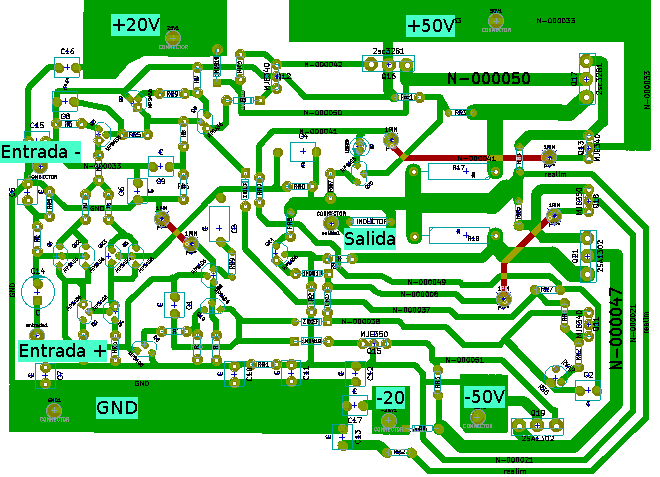
\includegraphics[width=\textwidth]{img/PCB1.png}
%\caption{Circuito impreso del amplificador.}
%\end{figure}

\subsubsection*{Reglas generales de dibujo}

El circuito tiene una área efectiva lo más pequeña posible con pistas tal que se minimizan las capacidades parásitas entre masa y las pistas de señal.
Queremos que las conexiones de masa y alimentación no tengan bucles. Para ello, intentamos de evitar los bucles y las pistas paralelas de mucha longitud y la cercanía entre ellas.
Las líneas de señal encierran la menor área posible compatible con la distribución de los elementos en su camino de retorno, cuidando especialmente los caminos de alta corriente y/o tensión de las líneas de gran sensibilidad.
Para disminuir el ruido hemos intentado evitar los puentes en la medida de lo posible, reduciéndolos a 3.

\subsubsection*{Repartición general}
La geometria del circuito respeta lo mejor posible las etapas originales del amplificador de potencia.  Esta disposición permite progeter la señal de entrada la cual es una de las mas débiles en tensión. De hecho, cuidamos que la entrada no sea mezclada con otras pistas de mayor corriente como por ejemplo la alimentacion, para evitar la inducción de ruido. Para eso tambien separamos las masas del circuito en dos lazos que se juntan en un punto unico, separando asi el camino de la corriente de alimentación del camino de la señal.
Este dibujo le permite tambien a juntar los transistores que calentan lo que permite de compartir los disipadores.

%\begin{figure}[H]
%\centering
%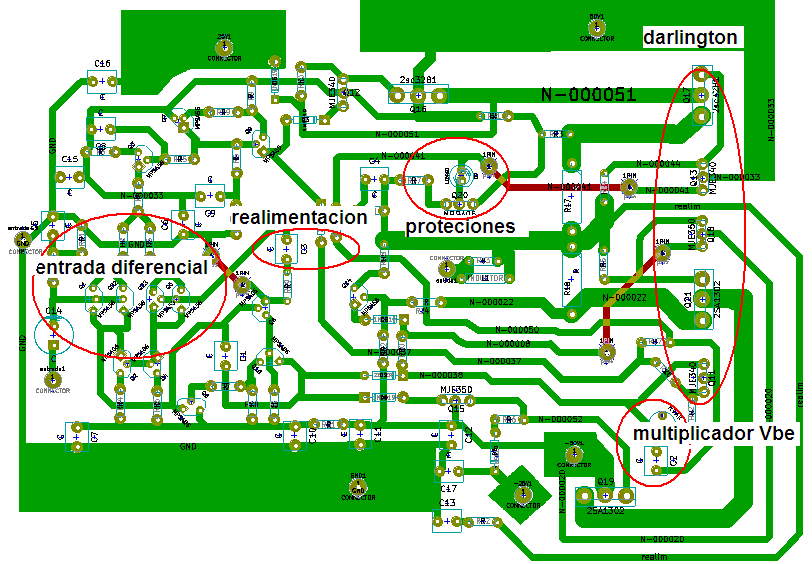
\includegraphics[width=\textwidth]{img/PCB2.png}
%\caption{Circuito impreso del amplificador.}
%\end{figure}

\subsubsection*{Alimentación}
Caminos de los conductores de alimentación suficientemente anchos y  dispuestos uno próximo al otro, con el objetivo de disminuir el área efectiva y por lo tanto la impedancia. Además, al estar cerca los caminos positivos y los negativos y no atravesar el circuitos, su campo eléctrico no afecta al resto.
También hicimos un plano de masa en estrella, para no concatenar ruido, con una parte dedicada a la entrada y la otra a la salida. Esto permite disminuir el ruido y proteger la señal de entrada.
 Agregamos después los capacitores de desacople del valor adecuado, de modo que funcionen a la frecuencia correspondiente. Lo hacemos lo más cerca del componente alimentado que sea posible.

\subsubsection*{Los resistencias en el emisor de salida}
Estas dos resistencias son de baja R y es importante que no se vean muy alteradas. Para evitar el cambio de temperatura hemos cuidado a que ninguna pista pasa debajo de estas dos resistencias. Además, los caminos que las conectan con la salida son anchos y perfectamente simétricos. De ésta forma, las pistas no sólo incorporan poca resistencia en serie sino que además, la incorporan en igual magnitud, cuestión de no perder la simetría a la salida, y que la degeneración de los transistores de salida sea lo mas simétrica posible.

\begin{figure}[H]
\centering
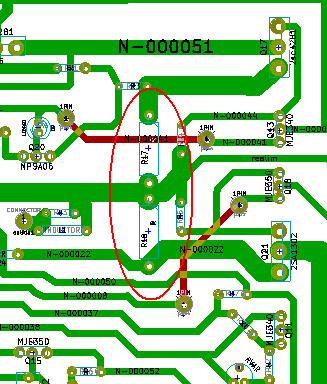
\includegraphics[scale=1]{img/PCB3.png}
\caption{Circuito impreso del amplificador.}
\end{figure}

\subsubsection{Disipadores}
\bigskip
Para el calculo de los disipadores se utilizo la ley experimental:
$$
   \theta_{ja}=\dfrac{T_{jm}-T_a}{P_D}
$$
$$
	\theta_{ja}=\theta_{jc}+\theta_{cs}+\theta_{sa}
$$

En la cual $\theta_{ja}$ es la resistencia térmica juntura-ambiente. Para cada transistor que maneje altas corrientes se calcula el valor del disipador requerido teniendo en cuenta la potencia disipada y su resistencia térmica. En el caso del transistor del multiplicador Vbe, que requiere estar a la misma temperatura que los de la salida clase B, se ubicará en el mismo disipador para disminuir la diferencia de temperaturas entre ellos.

\subsubsection{Circuito Implementado}
\begin{figure}[H]
\centerline{
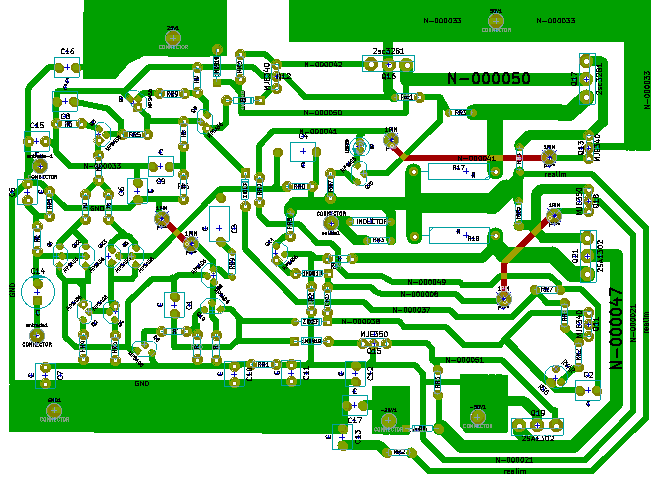
\includegraphics[width=1\textwidth]{img/circuito_implementado_todo.png}}
\caption{Circuito impreso del amplificador.}
\end{figure}

\subsubsection{Fuente Lineal}
\medskip
Para este circuito se utilizaron pistas de 4mm de ancho. Los diodos utilizados en el puente son 6A10 los cuales pueden soportar las corrientes requeridas por el amplificador, ya que soportan hasta 6A; y poseen una caída de tension en directa menor a 1V.
En la Figura~\ref{circuito_impreso_fuente_lineal} se muestra el circuito impreso implementado. 

\begin{figure}[H]
\centering
\centerline{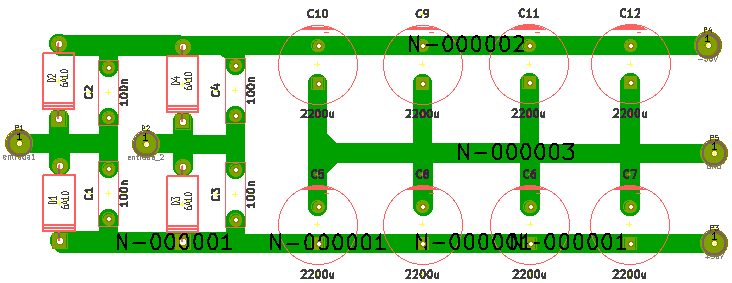
\includegraphics[width=1\textwidth]{img/circuito_impreso_fuente_lineal.png}}
\caption{Circuito impreso de la fuente lineal.}
\label{circuito_impreso_fuente_lineal} 
\end{figure}
\medskip
\subsubsection{Preamplificador}

En este impreso se debió tener en cuenta las posiciones y sentido de giro de los potenciometros para lograr un frente coherente y ordenado. Se agrego un conector jack a la salida para facilitar la desconexión con el amplificador de potencia de ser necesario.
Se utilizaron amplificadores operacionales NE5532, típicos en este tipo de aplicaciones debido a sus buenas prestaciones y bajo ruido.

\begin{figure}[H]
\centering
\centerline{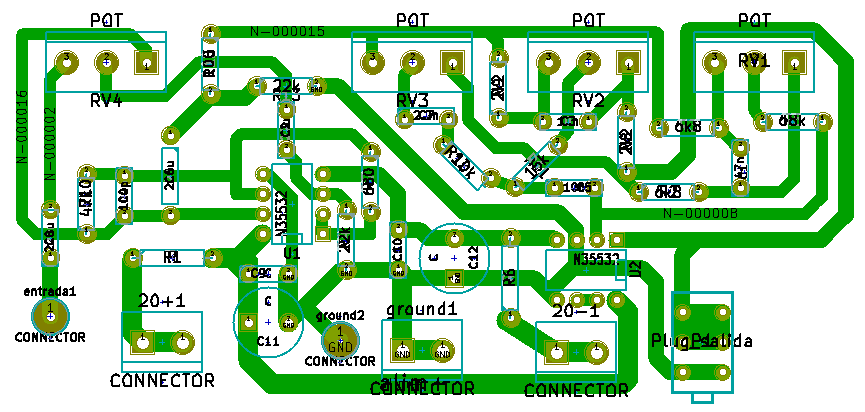
\includegraphics[width=1\textwidth]{img/pre_pcb.png}}
\caption{Circuito impreso del preamplificador.}
\label{pre_pcb} 
\end{figure}